\documentclass{beamer}
\usetheme{metropolis}

\usepackage[utf8]{inputenc}
\usepackage[ngerman]{babel}                                 % deutsche Sprache
\usepackage[T1]{fontenc}                                    % Unterstützung für Umlaute mit Fonts
\usepackage[autostyle=true,german=quotes]{csquotes}			% Wird für den Befehl \enquote benötigt
\usepackage{tikz}											% Ermöglicht das Zeichnen von Grafiken
\usepackage{amssymb}										% Einfügen von zusätzlichen Symbolen wie \square
\usepackage{enumitem}										% Erweiterte Funktionen der enumerate Umgebung
\usepackage{marvosym}										% Einfügen nützlicher Symbole

% Zeichnen von Darstellungen
\usepackage{tikz}
\usepackage{pgfplots}
\usepackage{pgfplotstable}
\usepackage{xcolor}

\usetikzlibrary{positioning,calc}

% Hinzufügen weiterer Symbole
\usepackage{bbding}

\metroset{titleformat=smallcaps,		% Überschriften werden in smallcaps geschrieben
	sectionpage=simple,					% Entfernen der Progressbar auf den Sectionpages
	block=fill,							% Hinterlegen von Umgebungen wie Theorem oder Example
}						

\definecolor{design1}{HTML}{639ACE}
\definecolor{design2}{HTML}{53972F}
\definecolor{design3}{HTML}{C33F4F}
\definecolor{design4}{HTML}{DC8C46}
\definecolor{design5}{HTML}{4A34A8}	

% Treffen von Einstellungen für tikz
\usetikzlibrary{positioning}
\usetikzlibrary{fit}
\usetikzlibrary{shapes.geometric}
\tikzset{main node/.style={circle,fill=blue!50,draw,minimum size=0.7cm,inner sep=0pt},}
\tikzset{bezier/.style={inner sep=0pt,minimum size=0cm},}


\title{Effiziente String-Verarbeitung in Datenbankanfragen auf hochgradig paralleler Hardware}
\subtitle{Masterarbeit}
\date{\today}
\author{Florian Lüdiger}
\institute{Fakultät Informatik - Lehrstuhl 6 - TU Dortmund}
\begin{document}
	\maketitle
	
	\section{Ein einfacher String-Vergleich auf der GPU}
	\begin{frame}{GPU-Verarbeitungsmodell}
		\begin{columns}[T] % align columns
			\begin{column}{.48\textwidth}				
				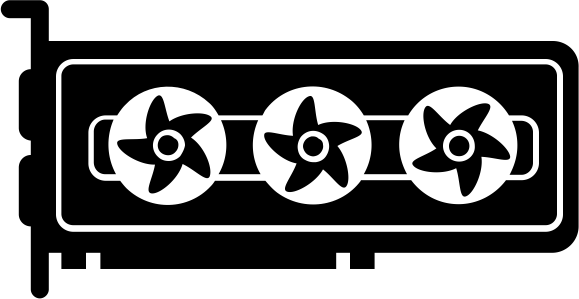
\includegraphics[width=100px]{grafikkarte.png}
				
				\huge
				NVIDIA GTX 950\\
				\normalsize
				\vspace{0.5\baselineskip}
				768 CUDA-Cores,\\
				2GB Speicher,\\
				6 Maxwell Streaming Multiprocessors,\\
				128 CUDA-Cores pro SMM
			\end{column}%
			\vrule
			\hfill%		
			\begin{column}{.48\textwidth}				
				\huge
				Warp Scheduling\\
				\normalsize
				\vspace{0.5\baselineskip}
				32 Threads = 1 Warp\\
				n Warps = 1 Block\\
				m Blocks = Grid\\
				\vspace{5em}
				\Large
				\textbf{Single Instruction,\\ Multiple Threads}
			\end{column}%
		\end{columns}
	\end{frame}
	\begin{frame}{String-Vergleich}
		\centering
		
		\tikzset{t_label/.style={rectangle,draw,minimum size=0.4cm,minimum width=2.1cm,inner sep=0pt}}
		\tikzset{t_length/.style={rectangle,draw,minimum size=0.4cm,inner sep=0pt,fill=blue!30}}
		\tikzset{t_active/.style={rectangle,draw,minimum size=0.4cm,inner sep=0pt}}
		\tikzset{t_inactive/.style={rectangle,draw,minimum size=0.4cm,inner sep=0pt,fill=black!30}}
		\tikzset{t_blank/.style={rectangle,minimum size=0.4cm,inner sep=0pt}}
		
		\begin{tikzpicture}
		\node (l1) {\textsf{Datensatz: OMA, OPA, OTTO | AHA, OMA, OHM |}};
		\node[below left = 0cm and -5.15cm of l1] (l2) {\textsf{OHA, DBMS, SQL}};
		\end{tikzpicture}
		
		\hfill
		
		\begin{tikzpicture}
		\begin{scope}
		\node[t_label] (0s) {\textsf{Suchstr.}};
		\node[t_label,below = 0.1cm of 0s] (0a) {\textsf{Thread 1}};
		\node[t_label,below = 0.1cm of 0a] (0b) {\textsf{Thread 2}};
		\node[t_label,below = 0.1cm of 0b] (0c) {\textsf{Thread 3}};
		
		\node[t_length, right = 0.3cm of 0s] (1s) {\textsf{3}};
		\node[t_length, right = 0.3cm of 0a] (1a) {\textsf{3}};
		\node[t_length, right = 0.3cm of 0b] (1b) {\textsf{3}};
		\node[t_length, right = 0.3cm of 0c] (1c) {\textsf{4}};
		
		\node[t_active, right = 0cm of 1s] (2s) {\textsf{O}};
		\node[t_active, right = 0cm of 1a] (2a) {\textsf{O}};
		\node[t_active, right = 0cm of 1b] (2b) {\textsf{O}};
		\node[t_inactive, right = 0cm of 1c] (2c) {};
		
		\node[t_active, right = 0cm of 2s] (3s) {\textsf{M}};
		\node[t_active, right = 0cm of 2a] (3a) {\textsf{M}};
		\node[t_active, right = 0cm of 2b] (3b) {\textsf{P}};
		\node[t_inactive, right = 0cm of 2c] (3c) {};
		
		\node[t_active, right = 0cm of 3s] (4s) {\textsf{A}};
		\node[t_active, right = 0cm of 3a] (4a) {\textsf{A}};
		\node[t_inactive, right = 0cm of 3b] (4b) {};
		\node[t_inactive, right = 0cm of 3c] (4c) {};
		
		\node[t_blank, right = 0cm of 4s] (5s) {};
		\node[t_active, right = 0cm of 4a,fill=green!30] (5a) {\Checkmark};
		\node[t_active, right = 0cm of 4b,fill=red!30] (5b) {\XSolid};
		\node[t_active, right = 0cm of 4c,fill=red!30] (5c) {\XSolid};
		
		\node[t_length, right = 0.1cm of 5s] (6s) {\textsf{3}};
		\node[t_length, right = 0.1cm of 5a] (6a) {\textsf{3}};
		\node[t_length, right = 0.1cm of 5b] (6b) {\textsf{3}};
		\node[t_length, right = 0.1cm of 5c] (6c) {\textsf{3}};
		
		\node[t_active, right = 0cm of 6s] (7s) {\textsf{O}};
		\node[t_active, right = 0cm of 6a] (7a) {\textsf{A}};
		\node[t_active, right = 0cm of 6b] (7b) {\textsf{O}};
		\node[t_active, right = 0cm of 6c] (7c) {\textsf{O}};
		
		\node[t_active, right = 0cm of 7s] (8s) {\textsf{M}};
		\node[t_inactive, right = 0cm of 7a] (8a) {};
		\node[t_active, right = 0cm of 7b] (8b) {\textsf{M}};
		\node[t_active, right = 0cm of 7c] (8c) {\textsf{H}};
		
		\node[t_active, right = 0cm of 8s] (9s) {\textsf{A}};
		\node[t_inactive, right = 0cm of 8a] (9a) {};
		\node[t_active, right = 0cm of 8b] (9b) {\textsf{A}};
		\node[t_inactive, right = 0cm of 8c] (9c) {};
		
		\node[t_blank, right = 0cm of 9s] (10s) {};
		\node[t_active, right = 0cm of 9a,fill=red!30] (10a) {\XSolid};
		\node[t_active, right = 0cm of 9b,fill=green!30] (10b) {\Checkmark};
		\node[t_active, right = 0cm of 9c,fill=red!30] (10c) {\XSolid};
		
		\node[t_length, right = 0.1cm of 10s] (11s) {\textsf{3}};
		\node[t_length, right = 0.1cm of 10a] (11a) {\textsf{3}};
		\node[t_length, right = 0.1cm of 10b] (11b) {\textsf{4}};
		\node[t_length, right = 0.1cm of 10c] (11c) {\textsf{3}};
		
		\node[t_active, right = 0cm of 11s] (12s) {\textsf{O}};
		\node[t_active, right = 0cm of 11a] (12a) {\textsf{O}};
		\node[t_inactive, right = 0cm of 11b] (12b) {};
		\node[t_active, right = 0cm of 11c] (12c) {\textsf{S}};
		
		\node[t_active, right = 0cm of 12s] (13s) {\textsf{M}};
		\node[t_active, right = 0cm of 12a] (13a) {\textsf{H}};
		\node[t_inactive, right = 0cm of 12b] (13b) {};
		\node[t_inactive, right = 0cm of 12c] (13c) {};
		
		\node[t_blank, right = 0cm of 13s] (14s) {};
		\node[t_active, right = 0cm of 13a,fill=red!30] (14a) {\XSolid};
		\node[t_active, right = 0cm of 13b,fill=red!30] (14b) {\XSolid};
		\node[t_active, right = 0cm of 13c,fill=red!30] (14c) {\XSolid};
		
		\node[above = 0.1cm of 1s] (arr1) {};
		\node[above = 0.1cm of 14s] (arr2) {};
		\draw[->, thick] (arr1) -- (arr2) node[midway, above] {{\large\textsf{Ausführungszeit}}};
		\end{scope}
		
		\begin{scope}
		\node[below = 0.5cm of 1c] (laenge) {\textsf{Längenvergleich}};
		\node[below = -0.2cm of 1c] (laenge_arrow) {};
		\draw [->] (laenge) -- (laenge_arrow);
		
		\node[below right = -0.2cm and -0.08cm of 5c] (neue_daten_arrow) {};
		\node[below = 1.3cm of neue_daten_arrow, align = center] (neue_daten) {\textsf{Ergebnis schreiben,} \\ \textsf{neue Daten laden}};
		\draw [->] (neue_daten) -- (neue_daten_arrow);
		
		\node[below = 0.5cm of 14c] (abbruch) {\textsf{frühzeitiger Abbruch}};
		\node[below = -0.2cm of 14c] (abbruch_arrow) {};
		\draw [->] (abbruch) -- (abbruch_arrow);
		\end{scope}
		\end{tikzpicture}
	\end{frame}
	\begin{frame}{Auslastung der GPU}
		\centering 
		
		\tikzset{t_label/.style={rectangle,draw,minimum size=0.4cm,minimum width=2.1cm,inner sep=0pt,color=black!30}}
		\tikzset{t_length/.style={rectangle,draw,minimum size=0.4cm,inner sep=0pt,color=black!30}}
		\tikzset{t_active/.style={rectangle,draw,minimum size=0.4cm,inner sep=0pt,fill=green!50}}
		\tikzset{t_check/.style={rectangle,draw,minimum size=0.4cm,inner sep=0pt,color=black!30}}
		\tikzset{t_inactive/.style={rectangle,draw,minimum size=0.4cm,inner sep=0pt,fill=red!50}}
		\tikzset{t_blank/.style={rectangle,minimum size=0.4cm,inner sep=0pt,color=black!30}}
		
		\begin{tikzpicture}
		\begin{scope}
		\node[t_label] (0s) {\textsf{Suchstr.}};
		\node[t_label,below = 0.1cm of 0s] (0a) {\textsf{Thread 1}};
		\node[t_label,below = 0.1cm of 0a] (0b) {\textsf{Thread 2}};
		\node[t_label,below = 0.1cm of 0b] (0c) {\textsf{Thread 3}};
		
		\node[t_length, right = 0.3cm of 0s] (1s) {\textsf{3}};
		\node[t_length, right = 0.3cm of 0a] (1a) {\textsf{3}};
		\node[t_length, right = 0.3cm of 0b] (1b) {\textsf{3}};
		\node[t_length, right = 0.3cm of 0c] (1c) {\textsf{4}};
		
		\node[t_check, right = 0cm of 1s] (2s) {\textsf{O}};
		\node[t_active, right = 0cm of 1a] (2a) {\textsf{O}};
		\node[t_active, right = 0cm of 1b] (2b) {\textsf{O}};
		\node[t_inactive, right = 0cm of 1c] (2c) {};
		
		\node[t_check, right = 0cm of 2s] (3s) {\textsf{M}};
		\node[t_active, right = 0cm of 2a] (3a) {\textsf{M}};
		\node[t_active, right = 0cm of 2b] (3b) {\textsf{P}};
		\node[t_inactive, right = 0cm of 2c] (3c) {};
		
		\node[t_check, right = 0cm of 3s] (4s) {\textsf{A}};
		\node[t_active, right = 0cm of 3a] (4a) {\textsf{A}};
		\node[t_inactive, right = 0cm of 3b] (4b) {};
		\node[t_inactive, right = 0cm of 3c] (4c) {};
		
		\node[t_blank, right = 0cm of 4s] (5s) {};
		\node[t_check, right = 0cm of 4a] (5a) {\Checkmark};
		\node[t_check, right = 0cm of 4b] (5b) {\XSolid};
		\node[t_check, right = 0cm of 4c] (5c) {\XSolid};
		
		\node[t_length, right = 0.1cm of 5s] (6s) {\textsf{3}};
		\node[t_length, right = 0.1cm of 5a] (6a) {\textsf{3}};
		\node[t_length, right = 0.1cm of 5b] (6b) {\textsf{3}};
		\node[t_length, right = 0.1cm of 5c] (6c) {\textsf{3}};
		
		\node[t_check, right = 0cm of 6s] (7s) {\textsf{O}};
		\node[t_active, right = 0cm of 6a] (7a) {\textsf{A}};
		\node[t_active, right = 0cm of 6b] (7b) {\textsf{O}};
		\node[t_active, right = 0cm of 6c] (7c) {\textsf{O}};
		
		\node[t_check, right = 0cm of 7s] (8s) {\textsf{M}};
		\node[t_inactive, right = 0cm of 7a] (8a) {};
		\node[t_active, right = 0cm of 7b] (8b) {\textsf{M}};
		\node[t_active, right = 0cm of 7c] (8c) {\textsf{H}};
		
		\node[t_check, right = 0cm of 8s] (9s) {\textsf{A}};
		\node[t_inactive, right = 0cm of 8a] (9a) {};
		\node[t_active, right = 0cm of 8b] (9b) {\textsf{A}};
		\node[t_inactive, right = 0cm of 8c] (9c) {};
		
		\node[t_blank, right = 0cm of 9s] (10s) {};
		\node[t_check, right = 0cm of 9a] (10a) {\XSolid};
		\node[t_check, right = 0cm of 9b] (10b) {\Checkmark};
		\node[t_check, right = 0cm of 9c] (10c) {\XSolid};
		
		\node[t_length, right = 0.1cm of 10s] (11s) {\textsf{3}};
		\node[t_length, right = 0.1cm of 10a] (11a) {\textsf{3}};
		\node[t_length, right = 0.1cm of 10b] (11b) {\textsf{4}};
		\node[t_length, right = 0.1cm of 10c] (11c) {\textsf{3}};
		
		\node[t_check, right = 0cm of 11s] (12s) {\textsf{O}};
		\node[t_active, right = 0cm of 11a] (12a) {\textsf{O}};
		\node[t_inactive, right = 0cm of 11b] (12b) {};
		\node[t_active, right = 0cm of 11c] (12c) {\textsf{S}};
		
		\node[t_check, right = 0cm of 12s] (13s) {\textsf{M}};
		\node[t_active, right = 0cm of 12a] (13a) {\textsf{H}};
		\node[t_inactive, right = 0cm of 12b] (13b) {};
		\node[t_inactive, right = 0cm of 12c] (13c) {};
		
		\node[t_blank, right = 0cm of 13s] (14s) {};
		\node[t_check, right = 0cm of 13a] (14a) {\XSolid};
		\node[t_check, right = 0cm of 13b] (14b) {\XSolid};
		\node[t_check, right = 0cm of 13c] (14c) {\XSolid};
		
		\node[above = 0.1cm of 1s] (arr1) {};
		\node[above = 0.1cm of 14s] (arr2) {};
		\draw[->, thick, color=black!30] (arr1) -- (arr2) node[midway, above, color=black!30] {{\large\textsf{Ausführungszeit}}};
		\end{scope}
		\end{tikzpicture}
	\end{frame}
	\begin{frame}{Verbesserung durch das Lane Refill}
		\centering 
		
		\begin{tikzpicture}
		\node (x11) [draw,thick,minimum width=3,minimum height=3] {};
		\node (x12) [draw,thick,minimum width=3,minimum height=3, right = 0.5cm of x11] {};
		\node (x13) [draw,thick,minimum width=3,minimum height=3, right = 0.5cm of x12] {};
		\node (x14) [draw,thick,minimum width=3,minimum height=3, right = 0.5cm of x13] {};
		\node (x21) [draw,thick,minimum width=3,minimum height=3, below = 0.5cm of x11] {};
		\node (x22) [densely dashed, draw,thick,minimum width=3,minimum height=3, right = 0.5cm of x21] {};
		\node (x23) [draw,thick,minimum width=3,minimum height=3, right = 0.5cm of x22] {};
		\node (x24) [draw,thick,minimum width=3,minimum height=3, right = 0.5cm of x23] {};
		\node (x31) [densely dashed, draw,thick,minimum width=3,minimum height=3, below = 0.5cm of x21] {};
		\node (x32) [densely dashed, draw,thick,minimum width=3,minimum height=3, right = 0.5cm of x31] {};
		\node (x33) [draw,thick,minimum width=3,minimum height=3, right = 0.5cm of x32] {};
		\node (x34) [draw,thick,minimum width=3,minimum height=3, right = 0.5cm of x33] {};
		
		\node (x41) [draw,thick,minimum width=1,minimum height=1, below = 0.8cm of x31] {};
		\node (x42) [draw,thick,minimum width=3,minimum height=3, right = 0.5cm of x41] {};
		\node (x43) [draw,thick,minimum width=3,minimum height=3, right = 0.5cm of x42] {};
		\node (x44) [draw,thick,minimum width=3,minimum height=3, right = 0.5cm of x43] {};
		
		%buffer tuples
		\node (xb1) [draw,thick,minimum width=3,minimum height=3, right = 0.8cm of x44] {};
		\node (xb2) [draw,thick,minimum width=3,minimum height=3, below = 0.5cm of xb1] {};
		\node (xb3) [rotate=-90, below right = 0cm and 0.05cm of xb2] {\footnotesize $\cdots$};
		
		%buffer
		\node (rect) [draw, thick, minimum width = 0.7cm, minimum height = 2cm, below right = -0.7cm of xb1] {};
		\node[align=center, font=\footnotesize, rotate=-90, above right = 0.25cm and 0cm of rect] (b) {\textsf{divergence buffer}};
		
		%flush
		\coordinate [below = 0.2cm of x33] (fl1);
		\coordinate [below = 0.2cm of x34] (fl2);
		\coordinate [above = 0.38cm of rect] (fl3);
		
		\draw[->, thick] (x33) -- (fl1) -- (fl3) -- (rect);
		\draw[thick] (x34) -- (fl2);
		\node[align=center, font=\footnotesize, above left = 0cm of fl3] (b) {\textsf{flush}};
		
		%new elements
		\coordinate [above = 0.2cm of x41] (ne1);
		\coordinate [above = 0.2cm of x42] (ne2);
		\coordinate [above = 0.2cm of x43] (ne3);
		\coordinate [above = 0.2cm of x44] (ne4);
		\coordinate [left = 0.4cm of ne1] (ne5);
		
		
		\node (new) [above right = 0cm and -0.5cm of ne1] {\footnotesize \textsf{new elements}};
		\draw[->, thick] (ne1) -- (x41);
		\draw[->, thick] (ne2) -- (x42);
		\draw[->, thick] (ne3) -- (x43);
		\draw[->, thick] (ne5) -- (ne4) -- (x44);
		
		\node (x51) [densely dashed, draw,thick,minimum width=3,minimum height=3, below = 0.5cm of x41] {};
		\node (x52) [draw,thick,minimum width=3,minimum height=3, right = 0.5cm of x51] {};
		\node (x53) [draw,thick,minimum width=3,minimum height=3, right = 0.5cm of x52] {};
		\node (x54) [draw,thick,minimum width=3,minimum height=3, right = 0.5cm of x53] {};
		
		\node (x61) [densely dashed, draw,thick,minimum width=3,minimum height=3, below = 0.5cm of x51] {};
		\node (x62) [draw,thick,minimum width=3,minimum height=3, right = 0.5cm of x61] {};
		\node (x63) [draw,thick,minimum width=3,minimum height=3, right = 0.5cm of x62] {};
		\node (x64) [densely dashed, draw,thick,minimum width=3,minimum height=3, right = 0.5cm of x63] {};
		
		%refill 
		\coordinate [below = 0.2cm of x61] (rf1);
		\coordinate [below = 0.2cm of x64] (rf2);
		\coordinate [below = 0.23cm of rect] (rf3);
		\draw[->, thick] (rect) -- (rf3) -- (rf1) -- (x61);
		\draw[->, thick] (rf2) -- (x64);
		\node[align=center, font=\footnotesize, below left = 0cm of rf3] (b) {\textsf{refill}};
		
		\node (x71) [draw,thick,minimum width=3,minimum height=3, below = 0.5cm of x61] {};
		\node (x72) [draw,thick,minimum width=3,minimum height=3, right = 0.5cm of x71] {};
		\node (x73) [draw,thick,minimum width=3,minimum height=3, right = 0.5cm of x72] {};
		\node (x74) [draw,thick,minimum width=3,minimum height=3, right = 0.5cm of x73] {};
		
		\node[rotate=-90, below right = 0.2cm and 0.5cm of x72] (xend) {\LARGE $\cdots$};
		\node (ts) [left = 0.5cm of x11] {};
		\node (te) [left = 0.5cm of x71] {};
		\draw[->, thick] (ts) -- (te);
		\end{tikzpicture}
	\end{frame}

	\section{Paralleler Musterabgleich auf der GPU}

	\begin{frame}{NFA zum regulären Ausdruck \texttt{(0|1)*((00)+|001)0}}
		\centering 
		
		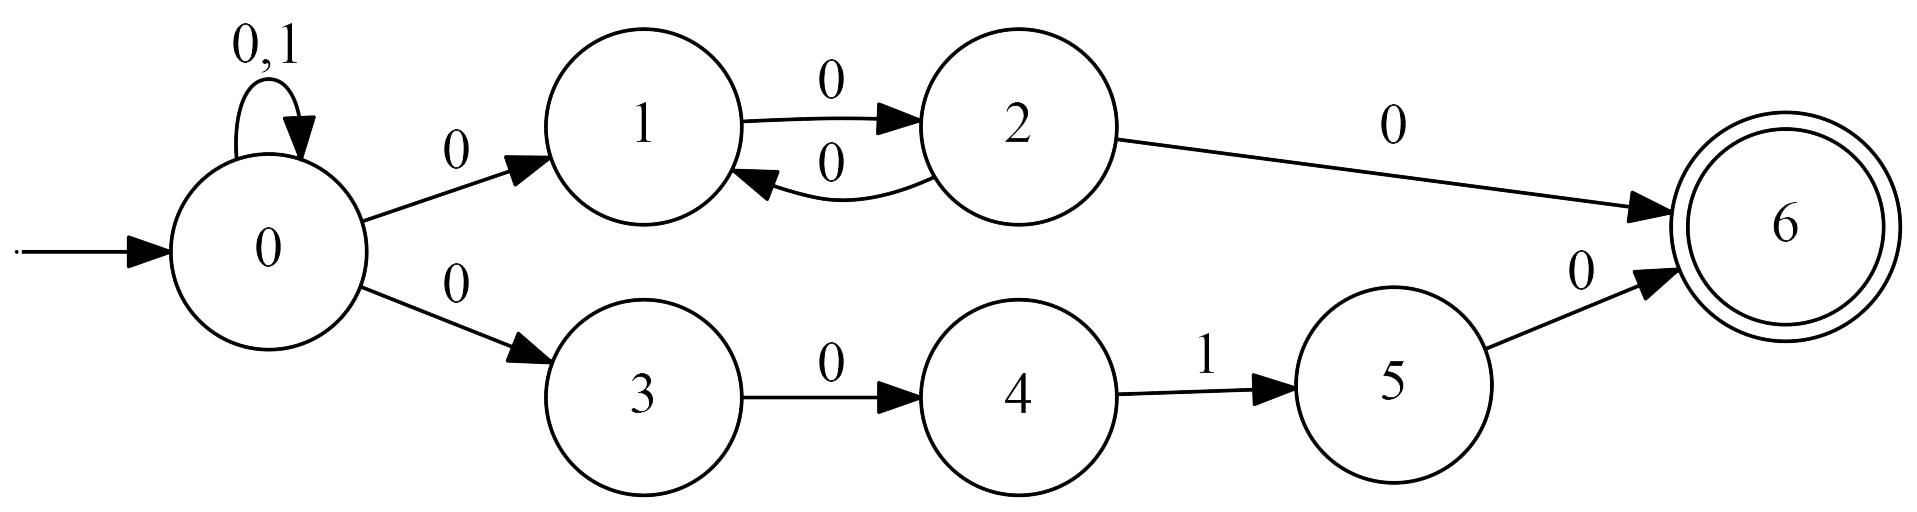
\includegraphics[width=\textwidth]{./nfa_beispiel.png}
		
		\vfill
		
		\begin{tabular}{ c | c c c c c c c}
			 & 0 & 1 & 2 & 3 & 4 & 5 & 6 \\
			\hline
			0 & 0,1,3 & 2 & 1,6 & 4 & - & 6 & - \\
			1 & 0 & - & - & - & 5 & - & - 
		\end{tabular}
	\end{frame}

	\begin{frame}{DFA zum regulären Ausdruck \texttt{(0|1)*((00)+|001)0}}
		\centering
		
		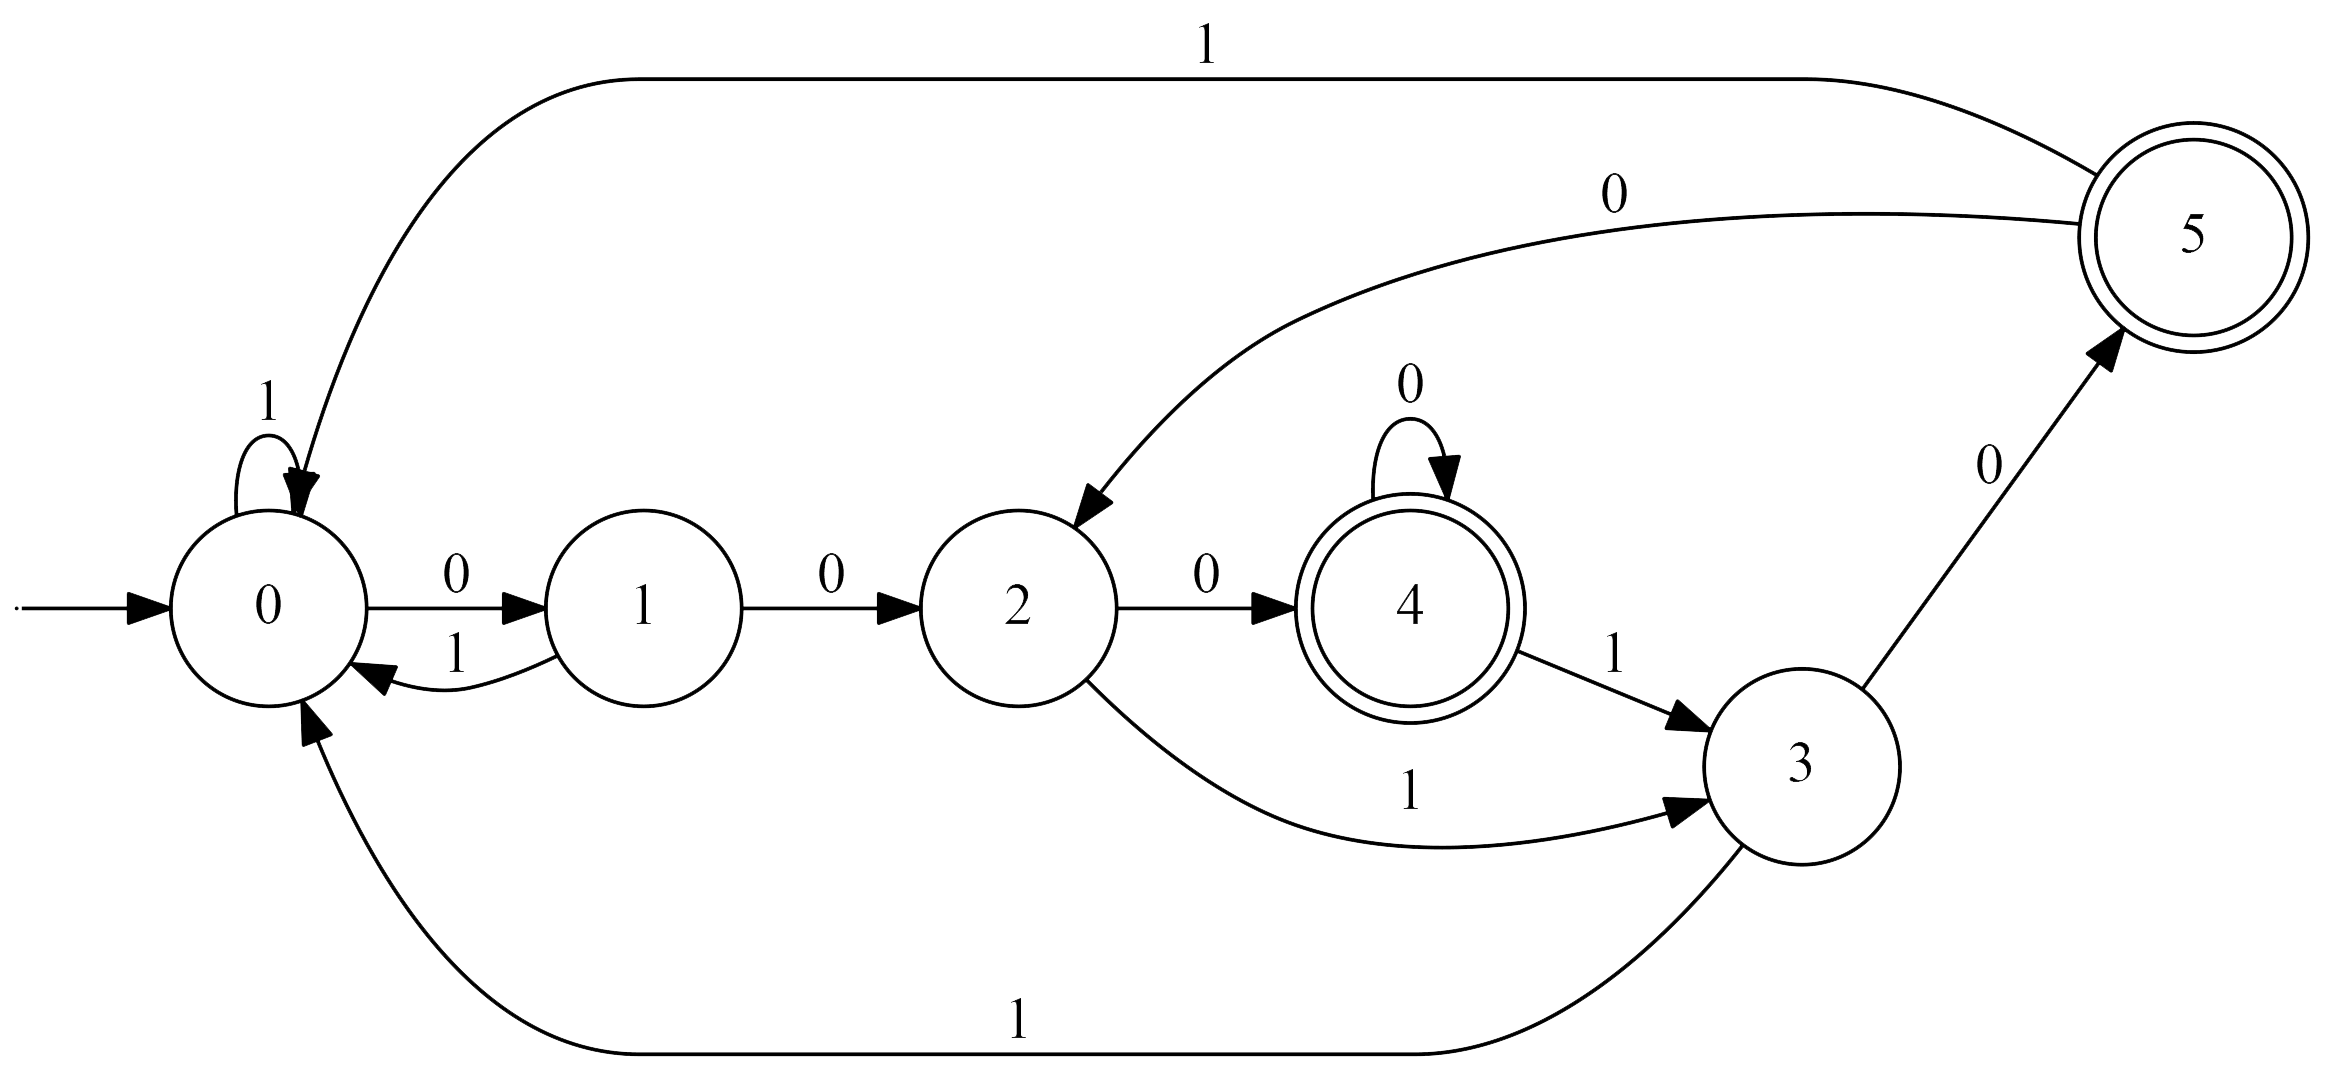
\includegraphics[width=\textwidth]{./dfa_beispiel.png}
		
		\vfill
		
		\begin{tabular}{c | c c c c c c}
			 & 0 & 1 & 2 & 3 & 4 & 5 \\
			\hline
			0 & 1 & 2 & 4 & 5 & 3 & 2 \\
			1 & 0 & 0 & 3 & 0 & 4 & 0
		\end{tabular}
	\end{frame}

	\section{Evaluation des einfachen String-Vergleichs}
	
	\begin{frame}{Gleichheitstest mit verschiedener Verteilung für Type-Daten}
		\begin{tikzpicture}[scale=0.7]
		\begin{axis}[
		ybar,		% Säulendiagramm
		xlabel={Anteil Matches},	% Achsenbeschriftung
		xtick=data,
		axis on top,
		xticklabels from table={../daten/type_equals.csv}{Selectivity},	% Beschriftung der Markierungen 
		width=450,	% Diagrammbreite
		height=330, % Diagrammhöhe
		bar width=0.2cm,	% Breite der Säulen
		ylabel={Laufzeit (ms)},	% Achsenbeschritung
		ymin=0,		% Säulen stehen auf der X-Achse
		%legend style={at={(0,0)}}
		legend pos=north west,		% Legende am oberen linken Rand positionieren
		legend style={legend cell align=left} % Text linksbündig anordnen
		]
		\addplot[fill=design1!60, draw=design1!70] table [x expr=\coordindex, y=equals]{../daten/type_equals.csv}; 
		\addlegendentry{Naiv};
		\addplot[fill=design2!60, draw=design2!70] table [x expr=\coordindex, y=buffer]{../daten/type_equals.csv};
		\addlegendentry{Mit Lane Refill}
		\addplot[fill=design3!60, draw=design3!70] table [x expr=\coordindex, y=unroll_2]{../daten/type_equals.csv};
		\addlegendentry{In Zweierschritten}
		\addplot[fill=design4!60, draw=design4!70] table [x expr=\coordindex, y=unroll_3]{../daten/type_equals.csv};
		\addlegendentry{In Dreierschritten}
		\end{axis}
		\end{tikzpicture}
	\end{frame}

	\begin{frame}{Präfixtest mit verschiedener Verteilung für Type-Daten}
		\begin{tikzpicture}[scale=0.7]
		\begin{axis}[
		ybar,		% Säulendiagramm
		xlabel={Anteil Matches},	% Achsenbeschriftung
		xtick=data,
		axis on top,
		xticklabels from table={../daten/type_prefix.csv}{Selectivity},	% Beschriftung der Markierungen 
		width=450,	% Diagrammbreite
		height=330, % Diagrammhöhe
		bar width=0.4cm,	% Breite der Säulen
		ylabel={Laufzeit (ms)},	% Achsenbeschritung
		ymin=0,		% Säulen stehen auf der X-Achse
		legend pos=north west,		% Legende am oberen linken Rand positionieren
		legend style={legend cell align=left} % Text linksbündig anordnen
		]
		\addplot[fill=design1!60, draw=design1!70] table [x expr=\coordindex, y=equals]{../daten/type_prefix.csv}; 
		\addlegendentry{Naiv};
		\addplot[fill=design2!60, draw=design2!70] table [x expr=\coordindex, y=buffer]{../daten/type_prefix.csv};
		\addlegendentry{Mit Lane Refill}
		\end{axis}
		\end{tikzpicture}
	\end{frame}

	\begin{frame}{Präfixtest mit verschiedener Verteilung für DBLP-Daten}
		\begin{tikzpicture}[scale=0.7]
		\begin{axis}[
		ybar,		% Säulendiagramm
		xlabel={Anteil Matches},	% Achsenbeschriftung
		xtick=data,
		axis on top,
		xticklabels from table={../daten/dblp_prefix.csv}{Selectivity},	% Beschriftung der Markierungen 
		width=450,	% Diagrammbreite
		height=330, % Diagrammhöhe
		bar width=0.4cm,	% Breite der Säulen
		ylabel={Laufzeit (ms)},	% Achsenbeschritung
		ymin=0,		% Säulen stehen auf der X-Achse
		legend pos=north west,		% Legende am oberen linken Rand positionieren
		legend style={legend cell align=left} % Text linksbündig anordnen
		]
		\addplot[fill=design1!60, draw=design1!70] table [x expr=\coordindex, y=equals]{../daten/dblp_prefix.csv}; 
		\addlegendentry{Naiv};
		\addplot[fill=design2!60, draw=design2!70] table [x expr=\coordindex, y=buffer]{../daten/dblp_prefix.csv};
		\addlegendentry{Mit Lane Refill}
		\end{axis}
		\end{tikzpicture}
	\end{frame}

	\section{Evaluation des parallelen Musterabgleichs}

	\begin{frame}{Präfixtest mit Basisalgorithmen für DBLP-Daten}
		\begin{tikzpicture}[scale=0.7]
		\begin{axis}[
		ybar,		% Säulendiagramm
		xlabel={Anteil Matches},	% Achsenbeschriftung
		xtick=data,
		axis on top,
		xticklabels from table={../daten/regex_dblpANY_no_buffer.csv}{Selectivity},	% Beschriftung der Markierungen 
		width=450,	% Diagrammbreite
		height=330, % Diagrammhöhe
		bar width=0.2cm,	% Breite der Säulen
		ylabel={Laufzeit (ms)},	% Achsenbeschritung
		ymin=0,		% Säulen stehen auf der X-Achse
		%legend style={at={(0,0)}}
		legend pos=north west,		% Legende am oberen linken Rand positionieren
		legend style={legend cell align=left} % Text linksbündig anordnen
		]
		\addplot[fill=design1!60, draw=design1!70] table [x expr=\coordindex, y=flat]{../daten/regex_dblpANY_no_buffer.csv}; 
		\addlegendentry{Flat};
		\addplot[fill=design2!60, draw=design2!70] table [x expr=\coordindex, y=table]{../daten/regex_dblpANY_no_buffer.csv};
		\addlegendentry{Table}
		\addplot[fill=design3!60, draw=design3!70] table [x expr=\coordindex, y=equals]{../daten/regex_dblpANY_no_buffer.csv};
		\addlegendentry{Präfix}
		\addplot[fill=design4!60, draw=design4!70] table [x expr=\coordindex, y=like]{../daten/regex_dblpANY_no_buffer.csv};
		\addlegendentry{Like}
		\end{axis}
		\end{tikzpicture}
	\end{frame}

	\begin{frame}{Verbesserungen durch das Lane Refill für DBLP-Daten}
		\begin{tikzpicture}[scale=0.7]
		\begin{axis}[
		ybar,		% Säulendiagramm
		xlabel={Anteil Matches},	% Achsenbeschriftung
		xtick=data,
		axis on top,
		xticklabels from table={../daten/regex_dblpANY_buffer.csv}{Selectivity},	% Beschriftung der Markierungen 
		width=450,	% Diagrammbreite
		height=330, % Diagrammhöhe
		bar width=0.2cm,	% Breite der Säulen
		ylabel={Verbesserung durch Lane Refill (\%)},	% Achsenbeschritung
		ymin=0,		% Säulen stehen auf der X-Achse
		%legend style={at={(0,0)}}
		legend pos=north west,		% Legende am oberen linken Rand positionieren
		legend style={legend cell align=left} % Text linksbündig anordnen
		]
		\addplot[fill=design1!60, draw=design1!70] table [x expr=\coordindex, y=flat]{../daten/regex_dblpANY_buffer.csv}; 
		\addlegendentry{Flat};
		\addplot[fill=design2!60, draw=design2!70] table [x expr=\coordindex, y=table]{../daten/regex_dblpANY_buffer.csv};
		\addlegendentry{Table}
		\addplot[fill=design3!60, draw=design3!70] table [x expr=\coordindex, y=equals]{../daten/regex_dblpANY_buffer.csv};
		\addlegendentry{Präfix}
		\end{axis}
		\end{tikzpicture}
	\end{frame}

	\begin{frame}{Optimierte Algorithmen mit DBLP-Daten}
		\begin{tikzpicture}[scale=0.7]
		\begin{axis}[
		ybar,		% Säulendiagramm
		xlabel={Anteil Matches},	% Achsenbeschriftung
		xtick=data,
		axis on top,
		xticklabels from table={../daten/regex_dblpANY_optimal.csv}{Selectivity},	% Beschriftung der Markierungen 
		width=450,	% Diagrammbreite
		height=330, % Diagrammhöhe
		bar width=0.2cm,	% Breite der Säulen
		ylabel={Laufzeit (ms)},	% Achsenbeschritung
		ymin=0,		% Säulen stehen auf der X-Achse
		%legend style={at={(0,0)}}
		legend pos=north west,		% Legende am oberen linken Rand positionieren
		legend style={legend cell align=left} % Text linksbündig anordnen
		]
		\addplot[fill=design1!60, draw=design1!70] table [x expr=\coordindex, y=flat-buffer]{../daten/regex_dblpANY_optimal.csv}; 
		\addlegendentry{Flat mit Lane Refill};
		\addplot[fill=design2!60, draw=design2!70] table [x expr=\coordindex, y=table-buffer]{../daten/regex_dblpANY_optimal.csv};
		\addlegendentry{Table mit Lane Refill}
		\addplot[fill=design3!60, draw=design3!70] table [x expr=\coordindex, y=equals-buffer]{../daten/regex_dblpANY_optimal.csv};
		\addlegendentry{Präfix mit Lane Refill}
		\addplot[fill=design4!60, draw=design4!70] table [x expr=\coordindex, y=like]{../daten/regex_dblpANY_optimal.csv};
		\addlegendentry{Like}
		\end{axis}
		\end{tikzpicture}
	\end{frame}

	\begin{frame}{Benchmark, der beliebige Anfangszeichen zulässt}
		\begin{tikzpicture}[scale=0.7]
		\begin{axis}[
		ybar,		% Säulendiagramm
		xlabel={Anteil Matches},	% Achsenbeschriftung
		xtick=data,
		axis on top,
		xticklabels from table={../daten/regex_ANYdblpANY.csv}{Selectivity},	% Beschriftung der Markierungen 
		width=450,	% Diagrammbreite
		height=330, % Diagrammhöhe
		bar width=0.15cm,	% Breite der Säulen
		ylabel={Laufzeit (ms)},	% Achsenbeschritung
		ymax=800,
		ymin=0,		% Säulen stehen auf der X-Achse
		%legend style={at={(0,0)}}
		legend pos=north east,		% Legende am oberen linken Rand positionieren
		legend style={legend cell align=left} % Text linksbündig anordnen
		]
		\addplot[fill=design1!60, draw=design1!70] table [x expr=\coordindex, y=flat]{../daten/regex_ANYdblpANY.csv}; 
		\addlegendentry{Flat};
		\addplot[fill=design2!60, draw=design2!70] table [x expr=\coordindex, y=flat-buffer]{../daten/regex_ANYdblpANY.csv};
		\addlegendentry{Flat mit Lane Refill}
		\addplot[fill=design3!60, draw=design3!70] table [x expr=\coordindex, y=table]{../daten/regex_ANYdblpANY.csv};
		\addlegendentry{Table}
		\addplot[fill=design4!60, draw=design4!70] table [x expr=\coordindex, y=table-buffer]{../daten/regex_ANYdblpANY.csv};
		\addlegendentry{Table mit Lane Refill}
		\addplot[fill=design5!60, draw=design5!70] table [x expr=\coordindex, y=like]{../daten/regex_ANYdblpANY.csv};
		\addlegendentry{Like}
		\end{axis}
		\end{tikzpicture}
	\end{frame}

	\begin{frame}{Unterschiedliche Automatengrößen mit TPC-H-Daten}
		\begin{tikzpicture}[scale=0.7]
		\begin{axis}[
		ybar,		% Säulendiagramm
		xlabel={Anzahl Zustände},	% Achsenbeschriftung
		xtick=data,
		axis on top,
		xticklabels from table={../daten/regex_p_name.csv}{states},	% Beschriftung der Markierungen 
		width=450,	% Diagrammbreite
		height=330, % Diagrammhöhe
		bar width=0.4cm,	% Breite der Säulen
		ylabel={Laufzeit (ms)},	% Achsenbeschritung
		ymin=0,		% Säulen stehen auf der X-Achse
		%legend style={at={(0,0)}}
		legend pos=north west,		% Legende am oberen linken Rand positionieren
		legend style={legend cell align=left} % Text linksbündig anordnen
		]
		\addplot[fill=design1!60, draw=design1!70] table [x expr=\coordindex, y=flat]{../daten/regex_p_name.csv}; 
		\addlegendentry{Flat};
		\addplot[fill=design2!60, draw=design2!70] table [x expr=\coordindex, y=flat-buffer]{../daten/regex_p_name.csv};
		\addlegendentry{Flat mit Lane Refill}
		\addplot[fill=design3!60, draw=design3!70] table [x expr=\coordindex, y=table]{../daten/regex_p_name.csv};
		\addlegendentry{Table}
		\addplot[fill=design4!60, draw=design4!70] table [x expr=\coordindex, y=table-buffer]{../daten/regex_p_name.csv};
		\addlegendentry{Table mit Lane Refill}
		\end{axis}
		\end{tikzpicture}
	\end{frame}
	
\end{document}